\documentclass[10pt]{article}
\usepackage{float}
\RequirePackage{eso-pic}
\usepackage{caption}
\captionsetup[table]{labelformat=empty}



\usepackage{geometry}
\geometry{
a4paper,
left=11mm,
right=14mm,
top=37mm,
bottom=14mm,
}



\usepackage{colortbl}
\usepackage{fontspec}
\setmainfont[Ligatures=TeX]{Calibri}



\newcommand\BackgroundPic{%
\put(0,0){%
\parbox[b][\paperheight]{\paperwidth}{%
\vfill
\centering
\includegraphics{MBIE_generic_background.pdf}%
\vfill
}}}



\begin{document}
\thispagestyle{empty}
\AddToShipoutPicture{\BackgroundPic}
\section*{Key Export Statistics\footnotemark - Onions\footnotemark }
\today\\
\begin{table}[ht]
\centering
{\scriptsize
\begin{tabular}[t]{p{1.8cm}>{\hfill}p{1.4cm}>{\hfill}p{1.4cm}>{\hfill}p{1.6cm}>{\hfill}p{1.9cm}>{\hfill}p{2cm}>{\hfill}p{1.9cm}>{\hfill}p{1.5cm}}
 \textbf{Country} & \textbf{Yearly Qty} & \textbf{Yearly Value} & \textbf{Yearly Price} & \textbf{3Year CAGR(Qty)} & \textbf{3Year CAGR(Value)} & \textbf{3Year CAGR(Price)} & \textbf{Price Elasticity} \\
\hline
Netherlands & 31,492 & 13.9 & \$0.4 & 7.8\% & 9.7\% & 1.7\% & 4.5 \\  
Indonesia & 21,307 & 10.2 & \$0.5 & 10\% & 22.5\% & 11.4\% & 0.9 \\  
Japan & 18,340 & 9.3 & \$0.5 & -9.9\% & -6.7\% & 3.6\% & -2.8 \\  
Germany & 15,764 & 6.4 & \$0.4 & 13\% & 24.3\% & 10\% & 1.3 \\  
Belgium & 14,348 & 6.2 & \$0.4 & 1.2\% & 6.1\% & 4.8\% & 0.2 \\  
Fiji & 8,675 & 5.2 & \$0.6 & 3.6\% & 16.8\% & 12.7\% & 0.3 \\  
Other & 59,838 & 30.2 & \$0.5 & -3.2\% & 4.1\% & 7.6\% & -0.4 \\  
Total & 169,765 & 81.5 & \$0.5 & 1\% & 7.2\% & 6.1\% & 0.2 \\  
\hline
\end{tabular}
}
\caption{\scriptsize Top 6 Onions Markets for year ending November - 2015: Quantity('000 kg) Value(NZ\$Mill), Price and their last 3-Year Growth Rates}
\end{table}


\vspace{-0.7cm}



   \begin{figure}[H]
   \centering
    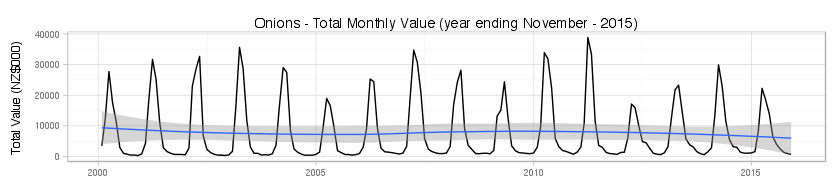
\includegraphics[scale=0.5]{../graphs/monthly_value/onions_monthly_value.png} \
    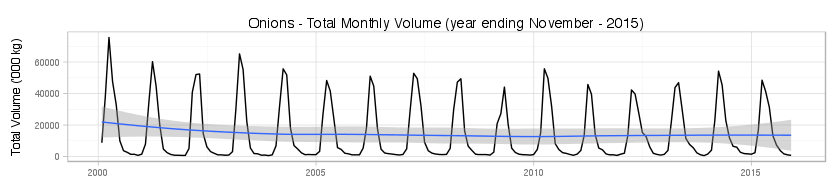
\includegraphics[scale=0.5]{../graphs/monthly_volume/onions_monthly_volume.png} \
    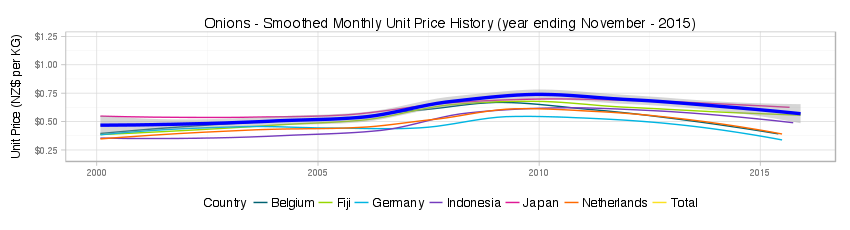
\includegraphics[scale=0.5]{../graphs/smoothed_price/onions_smoothed_price.png} \
    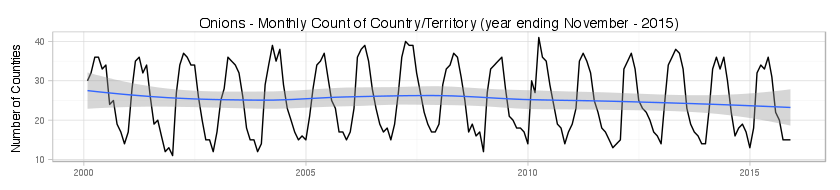
\includegraphics[scale=0.5]{../graphs/monthly_number_countries/onions_monthly_count.png} \
    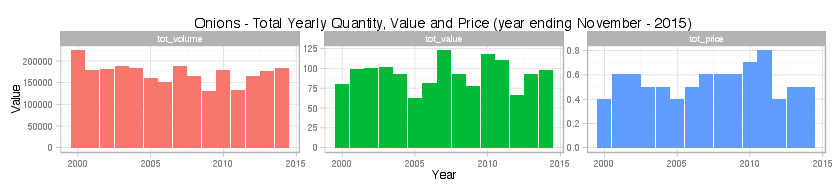
\includegraphics[scale=0.5]{../graphs/yearly_summary/onions_yearly_summary.png} \
   \end{figure}



\footnotetext[1]{Source: Statistics New Zealand - Overseas Merchandise Trade}
\footnotetext[2]{Harmonised System Codes for Onions starting with: 070310.}
\end{document}
